\addcontentsline{toc}{chapter}{Занятие 8. Случайные величины. Измеримость}
\chapter*{Занятие 8. Случайные величины. Измеримость}

\addcontentsline{toc}{section}{Контрольные вопросы и задания}
\section*{Контрольные вопросы и задания}

\subsubsection*{Приведите определение $ \sigma $-алгебры борелевых множеств, измеримой функции, болелевской функции, случайной величины, $ \sigma $-алгебры, порождённой случайной величиной.}

Борелевская $ \sigma $-алгебра --- наименьшая $ \sigma $-алгебра, порождённая открытыми множествами.

Пусть $ \left( X, \mathcal{F} \right) $ и $ \left( Y, \mathcal{G} \right) $ --- два множества с выделенными алгебрами подмножеств.
Тогда функция $f: X \rightarrow Y$ называется $ \mathcal{F} / \mathcal{G} $-измеримой, или просто измеримой,
если полный прообраз любого множества из $ \mathcal{G} $ принадлежит $ \mathcal{F} $, то есть
$$ \forall B \in \mathcal{G}, \,
f^{-1} \left( B \right) \in \mathcal{F},$$
где $f^{-1} \left( B \right) $ означает полный прообраз множества $B$.

Борелева (борелевская) функция:
$ \xi: \left( \mathbb{R}, \mathcal{B} \left( \mathbb{R} \right) \right) \rightarrow
\left( \mathbb{R}, \mathcal{B} \left( \mathbb{R} \right) \right) $.

Есть $ \left( \Omega, \mathcal{F} \right) $ --- пространство элементарных событий $ \Omega $ с $ \sigma $-алгеброй событий $ \mathcal{F} $ на нём.
Есть пара $ \left( \mathbb{R}, \mathcal{B} \left( \mathbb{R} \right) \right) $,
где $ \mathcal{B} \left( \mathbb{R} \right) - \sigma $-алгебра борелевых подмножеств на $ \mathbb{R} $.
Отображение $ \xi: \Omega \rightarrow \mathbb{R} $ называется случайной величиной, если выполняется $ \forall B \subset \mathcal{B} \left( \mathbb{R} \right): \, \left\{ \omega: \xi \left( \omega \right) \in B \right\} \in \mathcal{F} $, другими словами, $ \xi^{-1} \left( B \right) \in \mathcal{F} $ (прообраз каждого множества $B$ должен быть измеримым).

$ \sigma $-алгебра, порождённая случайной величиной $ \xi: X \rightarrow \mathbb{R} $, определяется следующим образом:
$$ \sigma \left( \xi \right) =
\left\{ \left. \xi^{-1} \left( B \right) \right| B \in \mathcal{B} \left( \mathbb{R} \right) \right\},$$
где $ \mathcal{B} \left( \mathbb{R} \right) $ --- борелевская сигма-алгебра на вещественной прямой.

\subsubsection*{Сформулируйте меру про сходимость по вероятности множеств из минимальной $ \sigma $-алгебры.}

Последовательность случайных величин $ \left\{ \xi_n: \, n \geq 1 \right\} $ сходится по вероятности к случайное величине $ \xi $, если:
$$ \forall \epsilon > 0, \qquad
P \left\{ \left| \xi_n - \xi \right| > \epsilon \right\} \rightarrow 0, \qquad
n \rightarrow \infty.$$

\subsubsection*{Какие $ \sigma $-алгебры называются независимыми?}

Пусть $ \mathcal{A}_1, \mathcal{A}_2 \subset \mathcal{F} $ две сигма-алгебры на одном и том же вероятностном пространстве.
Они называются независимыми, если любые их представители независимы между собой, то есть:
$$ \mathbb{P} \left( A_1 \cap A_2 \right) =
\mathbb{P} \left( A_1 \right) \cdot \mathbb{P} \left( A_2 \right), \qquad
\forall A_1 \in \mathcal{A}_1, \,
A_2 \in \mathcal{A}_2.$$

\subsubsection*{Приведите определение независимых случайных величин.}

Пусть дано семейство случайных величин $ \left( X_i \right)_{i \in I} $,
так что
$$X_i: \,
\Omega \rightarrow \mathbb{R}, \qquad
\forall i \in I.$$
Тогда эти случайные величины попарно независимы,
если попарно независимы порождённые ими сигма-алгебры $ \left\{ \sigma \left( X_i \right) \right\}_{i \in I} $.
Случайные величины независимы в совокупности, если таковы порождённые ими сигма-алгебры.

\addcontentsline{toc}{section}{Аудиторные задачи}
\section*{Аудиторные задачи}

\subsubsection*{8.3}

\textit{Задание.} Пусть $ \xi, \eta $ --- случайные величины, которые определены на вероятностном пространстве $ \left( \Omega, \mathcal{F}, \mathbb{P} \right) $.
Докажите,
что множества
$A = \\
= \left\{ \omega \in \Omega: \,
\xi \left( \omega \right) <
\eta \left( \omega \right) \right\}, \,
B =
\left\{ \omega \in \Omega: \,
\xi \left( \omega \right) =
\eta \left( \omega \right) \right\}, \,
C = \\
= \left\{ \omega \in \Omega: \,
\xi \left( \omega \right) \leq
\eta \left( \omega \right) \right\} $
являются событиями.

\textit{Решение.} Есть $ \xi, \eta $ --- случайные величины на вероятностном пространстве $ \left( \Omega, \mathcal{F}, \mathbb{P} \right) $.
Нужно доказать, что множества являются событиями, то есть они принадлежат $ \sigma $-алгебре $ \mathcal{F} $.

Нужно проверить, что
$$A =
\left\{ \omega \in \Omega: \,
\xi \left( \omega \right) <
\eta \left( \omega \right) \right\} \in
\mathcal{F}.$$

Пусть
$$ \forall c \in \mathbb{R}: \qquad \left\{ \omega: \xi \left( \omega \right) \leq c \right\} \in \mathcal{F}, \\
\forall b \in \mathbb{R}: \qquad \left\{ \omega: \xi \left( \omega \right) \leq b \right\} \in \mathcal{F}.$$

Множество вещественных чисел $ \mathbb{R} $ является несчётным.
Нужно счётное количество операций.
Может разделить две случайные величины рациональной точкой
\begin{equation*}
\begin{split}
A =
\bigcup \limits_{c_i \in \mathbb{Q} } \left\{ \omega \in \Omega: \, \xi \left( \omega \right) < c_i < \eta \left( \omega \right) \right\} = \\
= \bigcup \limits_{c_i \in \mathbb{Q} }
\left( \left\{ \omega \in \Omega: \, \xi \left( \omega \right) < c_i \right\} \cap
\left\{ \omega: \, \eta \left( \omega \right) > c_i \right\} \right).
\end{split}
\end{equation*}

С каждым множеством $ \sigma $-алгебра содержит дополнение.
Тогда
$ \\
\left\{ \omega: \, \eta \left( \omega \right) > b \right\} \in
\mathcal{F} $.
По условию
$$B =
\left\{ \omega \in \Omega: \,
\xi \left( \omega \right) =
\eta \left( \omega \right) \right\}.$$
Дополнение к нему равно
$$ \overline{B} =
\left\{ \omega \in \Omega: \,
\xi \left( \omega \right) >
\eta \left( \omega \right) \right\} \cup
\left\{ \omega \in \Omega: \,
\xi \left( \omega \right) <
\eta \left( \omega \right) \right\}.$$
По предыдущим пунктам каждое из этих множеств принадлежит $ \mathcal{F} $.
Из этого следует, чо объединение принадлежит $ \mathcal{F} $.

$C$ можно представить как
$$C =
A \cup B \in \mathcal{F},$$
так как $A \in \mathcal{F} $ и $B \in \mathcal{F} $.

\subsubsection*{8.4}

\textit{Задание.} Пусть $ \xi, \eta $ ---случайные величины, которые определены на вероятностном пространстве $ \left( \Omega, \mathcal{F}, \mathbb{P} \right) $.
Докажите, что следующие функции являются случайными величинами:
\begin{enumerate}[label=\alph*)]
\item $ \xi + \eta $;
\item $ \xi \cdot \eta $;
\item $ \max \left\{ \xi, \eta \right\} $. 
\end{enumerate}

\textit{Решение.} Если функция непрерывна, то она является измеримой.
В каждом случае $ \phi \left( \xi, \eta \right) $ --- случайная величина, если $ \phi $ --- непрерывная функция.
Тогда оно борелевская.

\subsubsection*{8.5}

\textit{Задание.}
Пусть $ \left( \Omega, \mathcal{F}, \mathbb{P} \right) $ ---
вероятностное пространство, $ \xi \left( \omega \right) $ --- действительнозначная функция, которая определена на $ \Omega $.
Должна ли $ \xi $ быть случайной величиной, если случайной величиной есть:
\begin{enumerate}[label=\alph*)]
\item $ \xi^2 $;
\item $ \left| \xi \right| $;
\item $ e^{ \xi } $. 
\end{enumerate}

\textit{Решение.} $ \xi $ --- случайная величина.
Отсюда следует, что $ \xi^2, \left| \xi \right|, e^{ \xi }$ --- случайные величины (взяли непрерывные функции).
В первых двух случаях будем строить контрпример, в третьем случае $ \xi $ будет случайной величиной.
Первые две функции не являются взаимно-однозначным отображением.
Третья --- взаимно-однозначное отображение (рис. \ref{fig:85}).

\begin{figure}[h!]
  \centering
  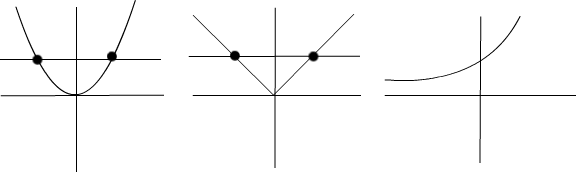
\includegraphics[width=.4\textwidth]{./pictures/8_5.png}
  \caption{Функции}
  \label{fig:85}
\end{figure}

\begin{enumerate}[label=\alph*)]
\item \item Строим контрпример.
Пусть
$$ \xi \left( \omega \right) =
\begin{cases}
1, \omega \in A, \\
-1, \omega \in \tilde{A},
\end{cases}$$
где $A$ --- измеримое множество, $ \tilde{A} $ --- не измеримое множество.
Тогда видим, что $ \xi $ не является случайной величиной, потому что
$$ \left\{ \omega: \,
\xi \left( \omega \right) =
- 1 \right\} =
\tilde{A} \in
\mathcal{F} $$
--- не измеримое множество ($ \sigma $-алгебра --- это только измеримые множества).
$$ \xi^2 \left( \omega \right) \equiv
1, \,
\left| \xi \left( \omega \right) \right| \equiv
1, \qquad
\forall \omega$$
\item $ e^{ \xi } $.
Тождественная единица --- это число (константа) --- случайная величина;
\item что значит, что $e^{ \xi }$ --- случайная величина?
$e^{ \xi }$ --- случайная величина.
Отсюда следует, что $ \forall c \in \mathbb{R}: \qquad \left\{ \omega: \, e^{ \xi \left( \omega \right) } \leq c \right\} $.
Можем записать, что это множество $ \left\{ \omega: \xi \left( \omega \right) \leq \ln c \right\} \in \mathcal{F} $, где $ \ln c \equiv d \in \mathbb{R} $.
Доказали, что для любого $d \in \mathbb{R} $ множество $ \left\{ \omega: \, \xi \left( \omega \right) \leq d \right\} \in \mathcal{F} $.
Тогда действительно $ \xi $ является случайной величиной. 
\end{enumerate}

\subsubsection*{8.6}

\textit{Задание.}
Пусть $ \left\{ \xi_n \right\}_{n \geq 1} $ ---
последовательность случайных величин, которые заданы на вероятностном пространстве $ \left( \Omega, \mathcal{F}, \mathbb{P} \right) $.
Докажите, что функции $ \inf \limits_{n} \xi_n, \, \sup \limits_{n} \xi_n $ являются случайными величинами.

\textit{Решение.} Нужно показать, что $ \forall c \in \mathbb{R}: \qquad \left\{ \omega: \, \inf \limits_{n} \xi_n \left( \omega \right) \leq c \right\} \in \mathcal{F} $.

Выписываем это множество и думаем, как его изобразить.
Хотя бы один элемент должен быть меньше $c$.
Отсюда следует, что
$$ \left\{ \omega: \,
\inf \limits_{n} \xi_n \left( \omega \right) \leq
c \right\} =
\bigcup \limits_{n=1}^{ \infty } \left\{ \omega: \,
\xi_n \left( \omega \right) \leq
c \right\}.$$
Каждое множество,
которое стоит под знаком объединения, по определению принадлежит $ \sigma $-алгебре $ \mathcal{F} $ и их счётное объединение принадлежит $ \sigma $-алгебре $ \mathcal{F} $.
$ \sigma $-алгебра замкнута относительно счётной операции объединения.
$$ \left\{ \omega: \,
\sup \limits_{n} \xi_n \left( \omega \right) >
c \right\} =
\bigcup \limits_{n=1}^{ \infty } \left\{ \omega: \,
\xi_n \left( \omega \right) > c \right\} \in
\mathcal{F}.$$
Это следует из того, что $\left\{ \omega: \, \xi_n \left( \omega \right) > c \right\} \in \mathcal{F} $, так как это случайная величина.

\subsubsection*{8.7}

\textit{Задание.} Пусть $ \left\{ \xi_n \right\}_{n \geq 1}$ --- последовательность случайных величин, которые определены на одном и том же вероятностном пространстве.
Докажите, что множества: $A = \left\{ \omega \in \Omega \; \middle| \; \right.$ последовательность $ \left\{ \xi_n \left( \omega \right) \right\}_{n \geq 1}$ ограничена\},
$B =
\left\{ \omega \in \Omega \; \middle| \; \xi_1 + \xi_2 \geq 5 \right\}, \,
C =
\left( \omega \in \Omega \; \middle| \; \xi_1 -3 \xi_2 \xi_3 + \xi_4^2 \cos \xi_1 \geq 0 \right\} $
являются случайными событиями.

\textit{Решение.} Чтоб доказать, что $A$ является случайной величиной, нужно показать, что $ \left\{ \omega \in \Omega \; \middle| \; \right. $ последовательность $ \left\{ \xi_n \left( \omega \right) \right\}_{n \geq 1}$ ограничена\} $ \in \mathcal{F} $ для произвольного $x \in \mathbb{R} $.

Последовательность $ \left\{ \xi_n \right\}_{n \geq 1}$ называется ограниченной, если она ограниченная сверху и ограниченная снизу, то есть существует такое число $x > 0$, что для любого номера $n, \left| \xi_n \left( \omega \right) \right| \leq x$.
Имеем: $ \left\{ \omega \in \Omega \; \middle| \; \right.$ последовательность $ \left\{ \xi_n \left( \omega \right) \right\}_{n \geq 1}$ ограничена\} $=
\bigcap \limits_{N=1}^{ \infty } \bigcup \limits_{n=1}^{ \infty }
\left\{ \omega \; \middle| \; \exists x > 0, \forall n, \qquad -x \leq \xi_n \left( \omega \right) \leq x \right\} = \\
= \bigcap \limits_{N=1}^{ \infty } \bigcup \limits_{n=1}^{ \infty }
\left\{ \omega \; \middle| \; \xi_n \left( \omega \right) \leq x \right\} \ \left\{ \omega \; \middle| \; \xi_n \left( \omega \right) < - x \right\} $.
Поскольку $ \xi_n $ является случайной,
то оба множества $ \left\{ \omega \; \middle| \; \xi_n \left( \omega \right) \leq x \right\} $ и
$ \left\{ \omega \; \middle| \; \xi_n \left( \omega \right) < - x \right\} $ принадлежат $ \sigma $-алгебре $ \mathcal{F} $,
а значит и их разница
$ \left\{ \omega \; \middle| \; \xi_n \left( \omega \right) \leq x \right\} \ \left\{ \omega \; \middle| \; \xi_n \left( \omega \right) < - x \right\} $
принадлежит этой $ \sigma $-алгебре.
Тогда и
$$ \bigcap \limits_{N=1}^{ \infty } \bigcup \limits_{n=1}^{ \infty }
\left\{ \omega \; \middle| \; \xi_n \left( \omega \right) \leq x \right\} \ \left\{ \omega \; \middle| \; \xi_n \left( \omega \right) < - x \right\} \in \mathcal{F}.$$


\addcontentsline{toc}{section}{Дополнительные задачи}
\section*{Дополнительные задачи}

\addcontentsline{toc}{section}{Домашнее задание}
\section*{Домашнее задание}

\subsubsection*{8.13}

\textit{Задание.} Пусть $A$ --- случайное событие.
Докажите, что
$$ \mathbbm{1}_A \left( \omega \right) =
\begin{cases}
1, \qquad \omega \in A, \\
0, \qquad \omega \notin A
\end{cases}$$
является случайной величиной.

\textit{Решение.}
Нужно доказать,
что $ \forall c \in \mathbb{R}, \qquad \left\{ \omega \; \middle| \; \mathbbm{1}_A \left( \omega \right) \leq c \right\} \in \mathcal{F} $,
где $ \mathcal{F} $ --- сигма-алгебра.

Пусть $c \geq 1$.
Тогда
$$ \left\{ \omega \; \middle| \;
\mathbbm{1}_A \left( \omega \right) \leq
c \right\} =
\Omega \in
\mathcal{F}.$$

В частности, при $c = 1$ получаем
$$ \left\{ \omega \; \middle| \;
\mathbbm{1}_A \left( \omega \right) \leq
1 \right\} =
\Omega \in
\mathcal{F},$$
так как по определению индикатора события он может принимать значение или 0, или 1, что всегда не больше единицы.
То есть неравенство справедливо для всех $ \omega $ из $ \Omega $.

По условию $A \in \mathcal{F}$.
По определению $ \sigma $-алгебры $ \overline{A} \in \mathcal{F} $.

Осталось доказать, что это выполняется и для $c < 1$.
Получаем множество
$$ \left\{ \omega \; \middle| \;
\mathbbm{1}_A < 1 \right\} =
\overline{A} \in \mathcal{F}.$$

Доказали, что соотношение выполняется для любого вещественного числа $c$.
Следовательно индикатор случайного события --- случайная величина.

\subsubsection*{8.14}

\textit{Задание.} Пусть $ \xi, \eta $ --- случайные величины, определённые на вероятностном пространстве $ \left( \Omega, \mathcal{F}, \mathbb{P} \right) $.
Докажите, что следующие функции являются случайными величинами:
\begin{enumerate}[label=\alph*)]
\item $ \xi - \eta $;
\item $ \min \left\{ \xi, \eta \right\} $;
\item $ \xi^{ \eta } $, где $ \xi $ --- положительная случайная величина.
\end{enumerate}

\textit{Решение.} Если функция непрерывна, то она является измеримой.

\begin{enumerate}[label=\alph*)]
\item
Чтобы доказать, что $ \xi - \eta $ является случайной величиной,
нужно показать, что $ \left\{ \omega \; \middle| \; \xi - \eta \leq x \right\} \in \mathcal{F} $ для произвольного $x \in \mathbb{R} $.
Имеем:
$$ \left\{ \omega \; \middle| \; \xi - \eta \leq x \right\} =
\left\{ \omega \; \middle| \; \xi \leq \eta + x \right\} =
\bigcup \limits_{n=1}^{ \infty } \left( \left\{ \omega \; \middle| \; \xi < r_n \right\} \cap
\left\{ \omega \; \middle| \; r_n < x - \eta \right\} \right),$$
где $ \left\{ r_n \right\} = \mathbb{Q} $.
Так как $ \xi $ и $ \eta $ являются случайными величинами,
то и множества
$ \left\{ \omega \; \middle| \; \xi < r_n \right\} $
и $ \left\{ \omega \; \middle| \; r_n < x - \eta \right\} $ принадлежат $ \sigma $-алгебре $ \mathcal{F} $,
а значит и их пересечение и объединение принадлежит этой $ \sigma $-алгебре;
\item нужно показать, что $ \left\{ \omega \; \middle| \; \min \left\{ \xi, \eta \right\} \leq x \right\} \in \mathcal{F} $ для произвольного $x \in \\
\in \mathbb{R} $.
Распишем
$ \left\{ \omega \; \middle| \; \min \left\{ \xi, \eta \right\} \leq x \right\} =
\left\{ \omega \; \middle| \; \xi \leq x \right\} \cup \left\{ \omega \; \middle| \; \eta \leq x \right\} $.
Так как $ \xi $ и $ \eta $ являются случайными величинами,
то и множества $ \left\{ \omega \; \middle| \; \xi \leq x \right\} $ и $ \left\{ \omega \; \middle| \; \eta \leq x \right\} $ принадлежат $ \sigma $-алгебре $ \mathcal{F} $, а значит и их объединение принадлежит этой $ \sigma $-алгебре;
\item нужно показать, что $ \left\{ \omega \; \middle| \; \xi^{ \eta } \leq x \right\} \in \mathcal{F} $ для произвольного $x \in \mathbb{R} $.
Распишем $ \left\{ \omega \; \middle| \; \xi^{ \eta } \leq x \right\} = \left\{ \omega \; \middle| \; \eta \cdot \ln \xi \leq \ln x \right\} $.

Покажем сначала, что $ \ln \xi $ --- случайная величина.
Имеем множество
$ \left\{ \omega \; \middle| \; \ln \xi \leq \ln x \right\} =
\left\{ \omega \; \middle| \; \ln \xi \leq x' \right\} \in
\mathcal{F} $.
Следовательно $ \ln \xi $ --- случайная величина.

Покажем, что квадрат случайной величины тоже является случайной величиной
$ \left\{ \omega: \xi \leq x \right\} =
\left\{ \xi^2 \leq x^2 = x' \right\} \in
\mathcal{F} $.

Вернёмся к основной задаче
\begin{equation*}
\begin{split}
\left\{ \omega \; \middle| \; \eta \cdot \ln \xi \leq \ln x \right\} = \\
= \left\{ \omega \; \middle| \;
\eta^2 + \frac{1}{4} \cdot 2 \eta \cdot \ln \xi + \xi^2 - \eta^2 + \frac{1}{4} \cdot 2 \eta \cdot \ln \xi - \xi^2 \leq \ln x \right\} = \\
= \left\{ \omega \; \middle| \; \left[ \left( \eta + \ln \xi \right)^2 - \left( \eta - \ln \xi \right)^2 \right] \cdot
\frac{1}{4} \leq \ln x \right\} = \\
= \left\{ \omega \; \middle| \; \left( \eta + \ln \xi \right)^2 - \left( \eta - \ln \xi \right)^2 \leq 4 \ln x \right\} = \\
= \left\{ \omega \; \middle| \; \left[ \eta - \left( - \ln \xi \right) \right]^2 -
\left[ \eta - \ln \xi \right]^2 \leq 4 \ln x \right\} \in \mathcal{F}.
\end{split}
\end{equation*}
Значит $ \xi^{ \eta } $ --- случайная величина.
\end{enumerate}

\subsubsection*{8.15}

\textit{Задание.}
Пусть $ \left( \Omega, \mathcal{F}, \mathbb{P} \right) $ ---
вероятностное пространство, $ \xi \left( \omega \right) $ --- действительнозначная функция, определённая на $ \Omega $.
Должна ли $ \xi $ быть случайной величиной, если случайной величиной есть:
\begin{enumerate}[label=\alph*)]
\item $ \cos \xi $;
\item $ \xi^{ \xi } $, где $ \xi $ --- положительная случайная величина.
\end{enumerate}

\textit{Решение.} Функции не являются взаимно-однозначными, поэтому $ \xi $ не будет случайной величиной.
 \begin{enumerate}[label=\alph*)]
\item Строим контрпример.
Пусть
$$ \xi \left( \omega \right) =
\begin{cases}
1, \qquad \omega \in A, \\
- 1, \qquad \omega \in \tilde{A},
\end{cases}
$$
где $A$ --- измеримое множество, $ \tilde{A} $ --- неизмеримое множество.
Тогда $ \xi $ не является случайной величиной,
потому что $ \left\{ \omega \; \middle| \; \xi \left( \omega \right) = - 1 \right\} = \\
= \tilde{A} \in \mathcal{F} $ ---
неизмеримое множество ($ \sigma $-алгебра --- это только измеримые множества);
\item строим контрпример.
Пусть
$$ \xi \left( \omega \right) =
\begin{cases}
0.45, \qquad \omega \in A, \\
0.25, \qquad \omega \in \tilde{A},
\end{cases}
$$
где $A$ --- измеримое множество, $ \tilde{A} $ --- неизмеримое множество.
Тогда $ \xi $ не является случайной величиной,
потому что $ \left\{ \omega \; \middle| \; \xi \left( \omega \right) = - 1 \right\} = \\
= \tilde{A} \in \mathcal{F} $ ---
неизмеримое множество ($ \sigma $-алгебра --- это только измеримые множества)
\end{enumerate}

\subsubsection*{8.16}

\textit{Задание.} Пусть $ \left\{ \xi_n \right\}_{n \geq 1} $ --- последовательность случайных величин, определённых на одном и том же вероятностном пространстве.
Докажите, что $ \varlimsup \limits_{n \rightarrow \infty } \xi_n $ является случайной величиной. 

\textit{Решение.}
Запишем верхний предел последовательности в виде $ \varlimsup \limits_{n \rightarrow \infty } \xi_n = \\
= \inf \limits_{m \geq 1} \sup \limits_{n \geq m} \xi_n$.

Считаем, что $ \sup \limits_{n \geq 1} \xi_n $ может принимать значение $+ \infty $,
тогда
$$ \left\{ \omega \; \middle| \; \eta \left( \omega \right) =
\sup \limits_{n \geq 1} \xi_n =
+ \infty \right\} \in \mathcal{F}.$$

Аналогично $ \inf \limits_{n \geq 1} \xi_n $ может принимать значение $- \infty $,
тогда
$$ \left\{ \omega \; \middle| \; \xi \left( \omega \right) =
\inf \limits_{n \geq 1} \xi_n =
- \infty \right\} \in \mathcal{F}.$$

Покажем, что $ \sup \limits_{n \geq 1} \xi_n $ --- случайная величина
\begin{equation*}
\begin{split}
\forall c \in \mathbb{R}, \qquad \left\{ \omega \; \middle| \; \eta \left( \omega \right) \leq c \right\} =
\left\{ \omega \; \middle| \; \sup \limits_{n \geq 1} \xi_n \left( \omega \right) \leq c \right\} = \\
= \left\{ \omega \; \middle| \; \forall n \geq 1, \qquad \xi_n \left( \omega \right) \leq c \right\} =
\bigcap \limits_{n=1}^{ \infty } \left\{ \omega \; \middle| \; \xi_n \left( \omega \right) \leq c \right\} \in \mathcal{F},
\end{split}
\end{equation*}
так как каждое из множеств принадлежит $ \mathcal{F} $.
Следовательно супремум случайных величин --- это случайная величина.

Покажем, что$ \inf \limits_{n \geq 1} \xi_n $ --- случайная величина
\begin{equation*}
\begin{split}
\forall c \in \mathbb{R}, \qquad \left\{ \omega \; \middle| \; \xi \left( \omega \right) \leq c \right\} =
\left\{ \omega \; \middle| \; \inf \limits_{n \geq 1} \xi_n \left( \omega \right) \leq c \right\} = \\
= \left\{ \omega \; \middle| \; \forall n \geq 1, \qquad \xi_n \left( \omega \right) \leq c \right\} =
\bigcup \limits_{n=1}^{ \infty } \left\{ \omega \; \middle| \; \xi_n \left( \omega \right) \leq c \right\} \in \mathcal{F},
\end{split}
\end{equation*}
так как каждое из множеств принадлежит $ \mathcal{F} $.
Следовательно инфимум случайных величин --- это случайная величина.

Из этого следует, что верхний предел последовательности случайных величин --- случайная величина.

\subsubsection*{8.17}

\textit{Задание.} Пусть $ \left\{ \xi_n \right\}_{n \geq 1} $ --- последовательность случайных величин, определённых на одном и том же вероятностном пространстве.
Докажите,
что множество
$A = \left\{ \omega \in \Omega \; \middle| \; \right. $ последовательность $ \left\{ \xi_n \right\}_{n \geq 1} \\
$ является монотонной \} является случайным событием.

\textit{Решение.} Чтобы доказать, что множество $A$ является случайным событием, нужно показать, что $A \in \mathcal{F} $.
Поскольку последовательность является монотонной, то:
\begin{equation*}
\begin{split}
A =
\left\{ \forall n \geq 1, \qquad \xi_n - \xi_{n-1} \leq 0 \right\} = \\
= \bigcap \limits_{n=1}^{ \infty } \left\{ \omega \in \Omega: \xi_n - \xi_{n-1} \leq 0 \right\} \cup \left\{ \omega \in \Omega: \xi_{n-1} - \xi_n \leq 0 \right\}.
\end{split}
\end{equation*}

Поскольку $ \xi_n - \xi_{n-1} $ является случайной величиной при произвольных $n$, то
$$ \bigcap \limits_{n=1}^{ \infty } \left\{ \omega \in \Omega: \xi_n - \xi_{n-1} \leq 0 \right\} \cup
\left\{ \omega \in \Omega: \xi_{n-1} - \xi_n \leq 0 \right\} \in \mathcal{F},$$
поскольку $ \mathcal{F} $ есть $ \sigma $-алгебра.
